\chapter{语义分析及符号表表计算}
\label{cha:yu_yi_fen_xi_ji_fu_hao_biao_biao_ji_suan_}

\section{实验设计}
\label{sec:shi_yan_she_ji_2}

\par 这一部分主要完成对于语法分析工具的进一步完善,包括语法树的构建,语义分析,符号表的计算以及错误检查。前一章的内容为整个编译器的实现打下了基础,而这一章则是整个编译器的核心部分,这一部分所实现的程序让编译器真正理解其所编译的程序的语法含义。

\subsection{语法树的构建}
\label{sub:yu_fa_shu_de_gou_jian_}

\begin{figure}[htpb]
    \centering
    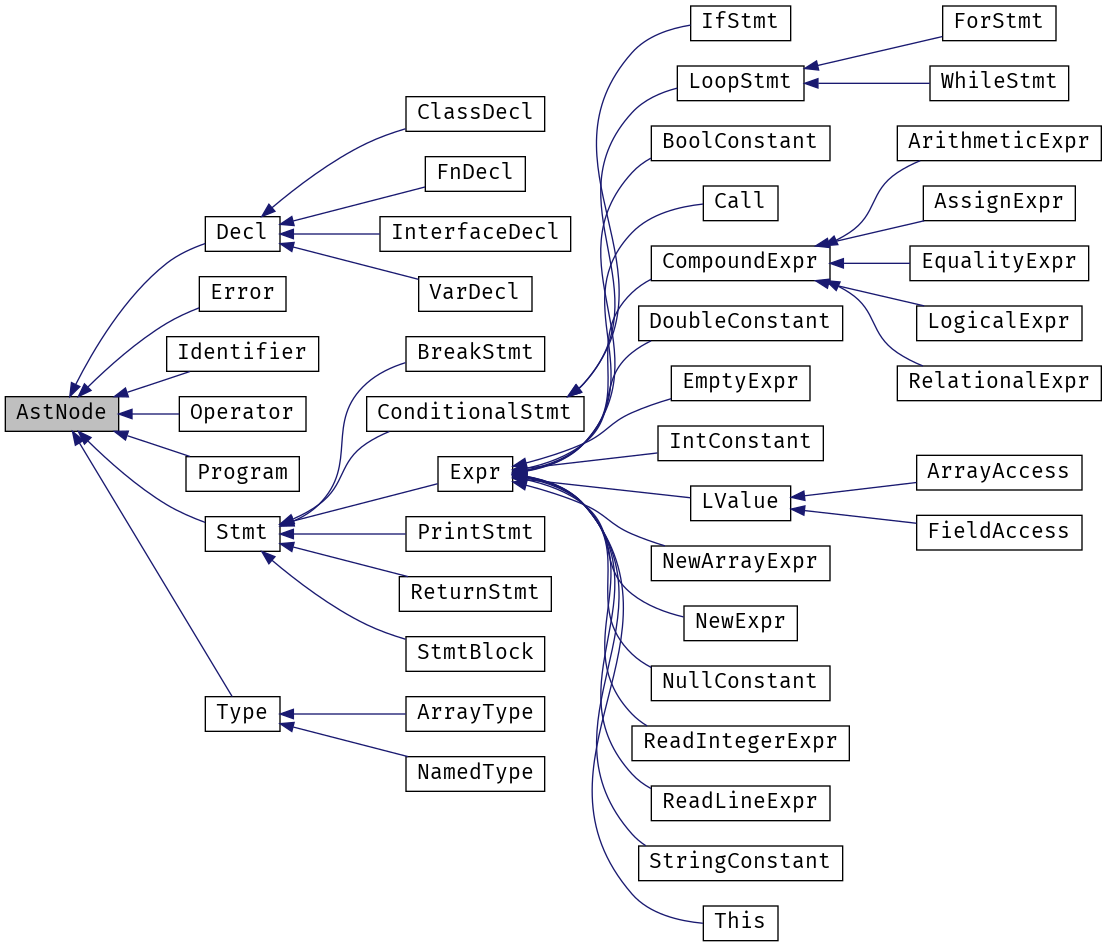
\includegraphics[width=0.78\textwidth]{struct.png}
    \caption{语法树节点类型继承树}
    \label{fig:struct}
\end{figure}

\par 首先进行的是语法树的构建,而这其中第一步则是对于语法树数据结构的设计。利用C++继承的特性,可以轻易地将语法树不同节点的共同特征以及可以应用于这些特征的共同方法提取出来。在最终的设计中决定采用一个AstNode类作为语法树所有节点类的基类,然后对于语法树中可能出现的类型进行继承细分,最终,的代的所有类型节点的继承继承关系如图\ref{fig:struct}所示。

\par 对于基类AstNode而言,其包含了所有语法树节点的基本特征:用于调试和错误处理的location成员,表示这个节点对应成员在源程序中的位置,一个指向父节点的指针,一个用于表示作用域的nodeScope成员以及一些节点通用方法,如在节点作用域内查找声明等。最终,生成的语法树的每一条边都是双向的,而指向子节点的指针则存放于各个继承的类中,每个类的子节点类型以及数量不同。
\par 为了在词法分析中能够正确的构建AST,需要将构建语法树的代码写入bison程序中。此后,由bison生成的词法分析程序来构建语法树。

\subsection{语义分析与错误处理}
\label{sub:yu_yi_fen_xi_}

\par 在语法树构建完成之后,接下来要进行的是静态语义分析。这一部保证了编写的语言在语义上是正确的。语法分析由节点类的check函数执行,每个节点的check函数负责检查自身是否符合语义限制。从根结点Program开始,第归地调用所有节点的check函数进行。check检查的范围包括流控制检查,唯一性检查、上下文检查(包括使用声明的检查以及作用域的检查)以及类型检查。注意类型检查是对于Expression(Expr类及其子类)进行的,Expr及其子类拥有checkAndCompureResultType()方法,通过check方法进行调用。这一方法不仅进行本节点的类型检查,还将本节点的类型计算并返回,用于上级表达式的类型检查。也就是说,类型计算在检查的过程中同时进行。

\par 在检查发现程序由错误时,根据不同的错误调用相应的函数进行报错。为了方便错误类型的管理,所有的报错过程均存储于ReportError类中,作为其静态方法存在,所有的报错均是通过这个类进行的。目前,程序能国处理的错误类型如表\ref{tab:error}所示。注意部分错误由词法分析器或语法分析器抛出,这些错误不再静态语义分析的范围内,但为了便于管理,也将这些错误处理函数置于本类内。

\begin{center}
    \begin{longtable}{r l l}
        \caption{错误类型及错误处理函数}
        \label{tab:error}\\ % NOTE THIS

        \toprule
        \multicolumn{1}{c}{\textbf{错误分类}} &
        \multicolumn{1}{c}{\textbf{错误分类}} &
        \multicolumn{1}{c}{\textbf{错误分类}} \\
        \cmidrule(lr){1-1} \cmidrule(lr){2-2} \cmidrule(lr){3-3}
        \endfirsthead

        \toprule
        \multicolumn{1}{c}{\textbf{错误分类}} &
        \multicolumn{1}{c}{\textbf{错误分类}} &
        \multicolumn{1}{c}{\textbf{错误分类}} \\
        \cmidrule(lr){1-1} \cmidrule(lr){2-2} \cmidrule(lr){3-3}
        \endhead

        \multirow{4}{*}{词法分析器错误}
        & UntermComment & 注释未结束 \\
        & LongIdentifier & 标识符过长 \\
        & UntermString & 字符串未结束 \\
        & UnrecogChar & 未知字符串 \\

        \cmidrule(lr){1-3}
        \multirow{3}{*}{声明相关错误}
        & DeclConflict & 声明冲突(重复声明)\\
        & OverrideMismatch & 方法重载签名不符 \\
        & InterfaceNotImplemented & 接口未实现 \\

        \cmidrule(lr){1-3}
        \multirow{1}{*}{标识符相关错误}
        & IdentifierNotDeclared & 标识符未声明 \\

        \cmidrule(lr){1-3}
        \multirow{3}{*}{表达式相关错误}
        & IncompatibleOperand & 运算符与又操作数不匹配 \\
        & IncompatibleOperands & 运算符与双操作数不匹配 \\
        & ThisOutsideClassScope & 类外使用this \\

        \cmidrule(lr){1-3}
        \multirow{3}{*}{数组相关错误}
        & BracketsOnNonArray & 对于非数组取地址 \\
        & SubscriptNotInteger & 数组下标不是整型 \\
        & NewArraySizeNotInteger & 使用NewArray时下标不是整型 \\

        \cmidrule(lr){1-3}
        \multirow{3}{*}{函数/方法相关错误}
        & NumArgsMismatch & 参数数量不匹配 \\
        & ArgMismatch & 参数类型不匹配 \\
        & PrintArgMismatch & 使用Print时参数类型不匹配 \\

        \cmidrule(lr){1-3}
        \multirow{2}{*}{域访问相关错误}
        & FieldNotFoundInBase & 为找到访问域 \\
        & InaccessibleField & 访问权限错误(如访问内部类成员) \\

        \cmidrule(lr){1-3}
        \multirow{3}{*}{流控制相关错误}
        & TestNotBoolean & 测试语句返回类型非bool \\
        & ReturnMismatch & return类型不匹配 \\
        & BreakOutsideLoop & 在循环外部使用break \\

        \cmidrule(lr){1-3}
        \multirow{1}{*}{链接错误}
        & NoMainFound & 主函数未找到 \\
        \bottomrule
    \end{longtable}
\end{center}

\subsection{符号表构建}
\label{sub:fu_hao_biao_gou_jian_}
\par 为了能够尽可能的减少遍历的次数,同时简化程序的逻辑,符号表的构建也在check中完成,并随着作用域分析(上下文相关性检查)的需要而惰性构建。
\par 符号表使用Hash表实现,封装于HashTable类中,而此类为stl中map容器的简单封装。每一个nodeScope成员(表示一个作用域)持有一张符号表,特殊节点Pogram持有全局符号表。符号表将标识符映射到声明节点,这样在查找符号的时候就可以通过声明节点进一步的动态查询所需要的信息,同时减少了符号表的负担,使之不需要存储过多的信息。
\par 在计算符号表时,由于符号表的计算时随着check函数而多心进行的,因此不需要第归进行计算,每次只需要计算本作用域的符号即可,随着check的进行而递归。对于每个scope所在的节点,采用declareAll注册其所有子节点的符号,并将其加入符号表中。为了方便调试,在注册符号的同时进行输出,而打印整个符号表。

\section{实验过程}
\label{sec:shi_yan_bu_zou_2}
\par 首先按照节点的继承树(图\ref{fig:struct})编写各个类型的节点的类定义。然后,将这些类加入语法分析其parser.y的union中,使得bison生成的程序能够将语法符号与类进行对应,从而执行相应的动作构建语法树。在编译与分分析器时,发现其不能正确的调用yylex进行词法分析。经过分析发现,由于在加入了语法树的构建后程序由gcc编译改为了g++编译以构建c++的类,从而导致yylex这一c函数不能正确被识别。在yylex的声明出加上\lstinline|extern "C"|后,问题得以解决。
\par 在修改完parser后能够正确的生成语法树了。然后修改每个节点的check函数以编写进行语义分析与检查的方法,值得注意的是,由于符号表计算随着语义分析中的上下文分析而惰性计算,但其他检查也可能用到符号表(如类型检查),因此符号表的计算必须在所有的检查前面完成。

\section{实验结果及分析}
\label{sec:shi_yan_jie_guo_ji_fen_xi_2}
\par 在程序编写完成后输入测试用程序1(见附录\ref{cha:ce_shi_yong_decafdai_ma_}),并对于输出进行分析。语法树构建的部分输出如图\ref{fig:syntaxTree}所示。将其结构与源程序进行比较,其结构与程序的结构一致,说明语法树在结构上时正确的。

\begin{figure}[htpb]
    \centering
    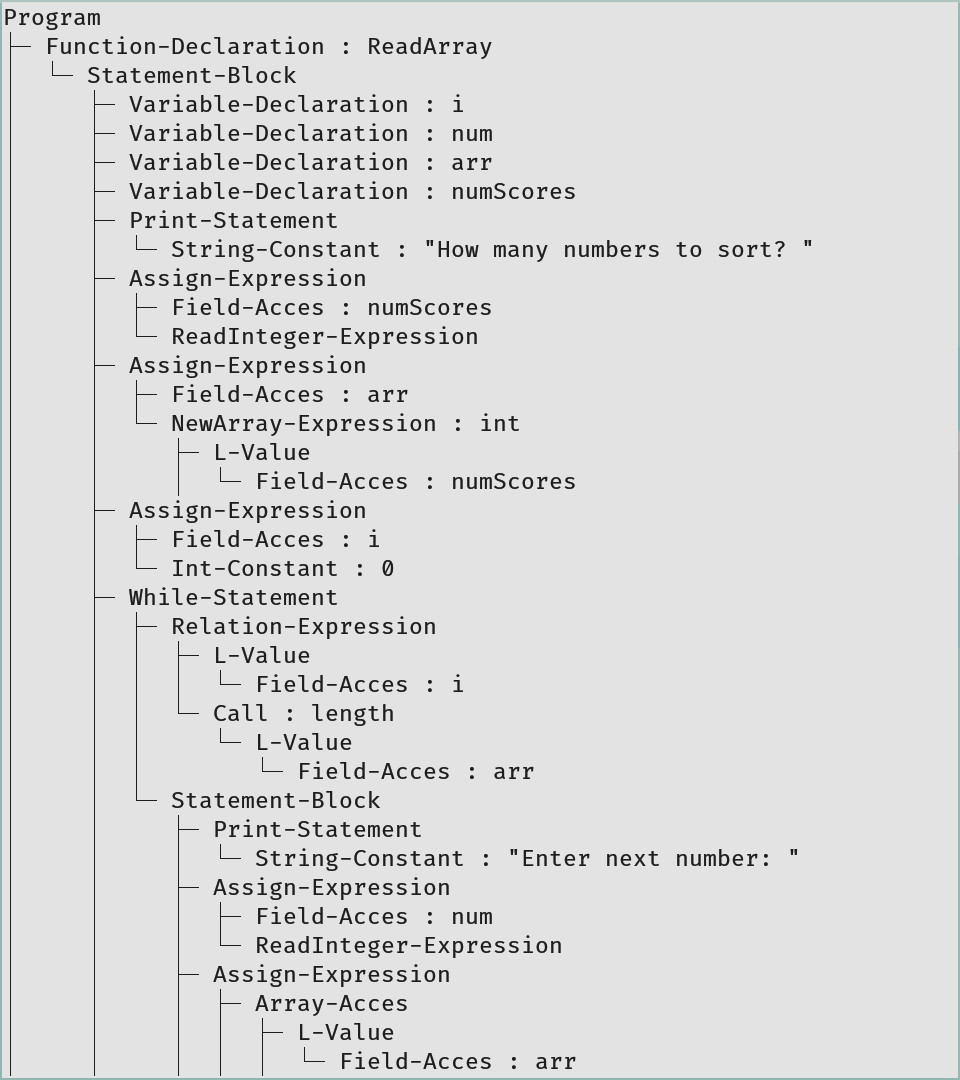
\includegraphics[width=0.8\linewidth]{syntaxTree.png}
    \caption{构建的语法树(部分)}
    \label{fig:syntaxTree}
\end{figure}

\par 然后,对于语法分析与错误处理进行测试。对于每一种错误,均编写了一个简短的程序进行测试,由于篇幅冗长不在此处全部放出,此处选择其中的一个样例错误程序进行测试:
\inputCodeSetLanguage{c++}
\begin{lstlisting}
void main(){
    int a;
    a=b+c;
    int b; int c;
}
\end{lstlisting}
\par 可以明显的看出,b和c在定义前被使用,此时程序应该汇报baddecl错误。程序的实际运行结果如图\ref{fig:baddecl}所示,可以看出,程序正确的汇报了baddecl错误并指出了错误的发生地点。对其他错误的测试表明程序的行为预期的一致,可以说明在定的错误范围内程序均能正常工作,识别并汇报对应的错误。
\begin{figure}[htpb]
    \centering
    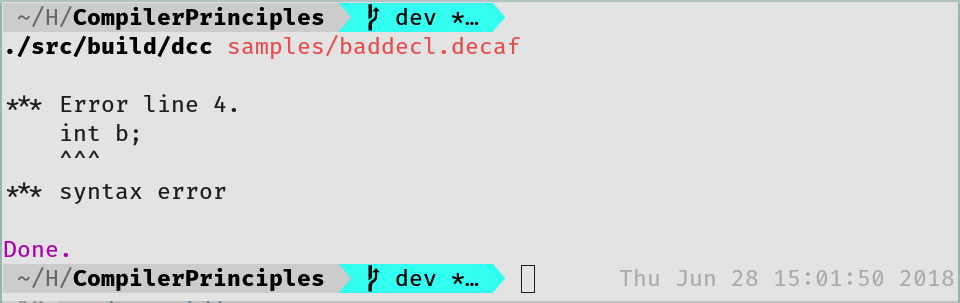
\includegraphics[width=0.74\linewidth]{baddecl.png}
    \caption{对于错误程序进行编译}
    \label{fig:baddecl}
\end{figure}

\par 最后,对符号表的输出进行观察,并与源程序进行比对,观察各个符号表所出现的作用域与作用域级别、类型是否与源程序中的一致。符号表以及作用域的输出如图\ref{fig:scope}所示。经过与源程序的比对后,确认了所有的符号均被录入,所对应的作用域以及级别也与人工分析的结果一致,从而推断符号表的构建是正确的。

\begin{figure}[htpb]
    \centering
    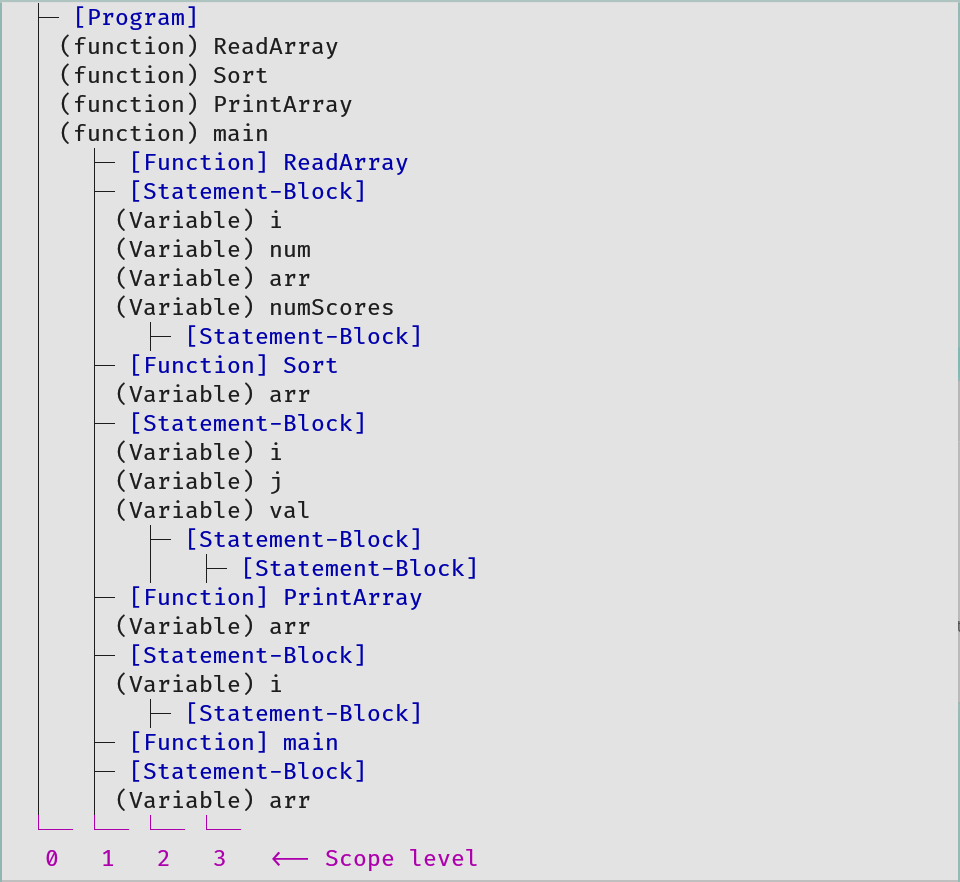
\includegraphics[width=0.74\linewidth]{scope.png}
    \caption{符号表与对应作用域输出}
    \label{fig:scope}
\end{figure}


